\chapter{Marco teórico}
\label{chap:marco-teorico}
% Versión 2 (2026-10-04). Conceptos estrictamente necesarios para la metodología del
% capítulo 3 integrado por la dirección (Overleaf, 2026-10-04; main 9558099). Depura la
% versión 1 de la propuesta. Notación idéntica a la del capítulo 3.

La metodología de este trabajo combina tres campos: la física del paso de los muones por la materia, la estadística de los procesos de conteo y el aprendizaje profundo aplicado a la mejora de imágenes. Este capítulo presenta los fundamentos de esos campos en el orden en que la metodología los requiere. Primero se explica por qué la atenuación del flujo de muones informa sobre la materia atravesada y qué contiene, y qué no contiene, una imagen muográfica por transmisión. Después se describe la estadística que gobierna su ruido, la simulación con la que pueden producirse imágenes de exposición conocida y los modelos capaces de estimar una imagen de mayor estadística a partir de una ruidosa. El capítulo concluye con los criterios con los que se juzga la calidad de esa estimación y con una revisión breve del aprendizaje profundo en muografía. Los procedimientos con los que estos conceptos se aplicaron se describen en el \cref{chap:metodologia}.

% =============================================================================
\section{Muones cósmicos y su paso por la materia}
\label{sec:mt-muones}

Los rayos cósmicos primarios, en su mayoría protones y núcleos de helio, interactúan con los núcleos de la alta atmósfera y producen cascadas de partículas secundarias. Entre ellas abundan los piones y kaones cargados, cuya desintegración da lugar a los muones. El muon tiene la carga del electrón y una masa de 105,7~MeV/$c^{2}$, unas doscientas veces mayor; no participa en la interacción fuerte y, por su masa, pierde energía por radiación mucho más lentamente que el electrón. Aunque su vida media en reposo es de 2,2~$\mu$s, la dilatación relativista del tiempo permite que una fracción importante de los muones producidos a decenas de kilómetros de altura alcance la superficie y atraviese después grandes espesores de roca \parencite{gaisser2016,pdg2022}.

El flujo en la superficie se describe por su intensidad diferencial $\Phi(E,\zeta)$, el número de muones por unidad de área, de tiempo, de ángulo sólido y de energía, que depende de la energía $E$ y del ángulo cenital $\zeta$ de la dirección de llegada. Al nivel del mar, la energía media de los muones es del orden de 4~GeV; el espectro es casi plano por debajo de 1~GeV y decae aproximadamente como $E^{-2{,}7}$ entre decenas y centenares de GeV. La intensidad disminuye con el ángulo cenital, en forma aproximadamente proporcional a $\cos^{2}\zeta$ para muones de algunos GeV, mientras que la energía media aumenta en las direcciones inclinadas, porque los muones de baja energía que recorren más atmósfera se desintegran o se detienen antes de llegar al suelo \parencite{pdg2022}. Para la muografía interesa el flujo integral por encima de un umbral de energía $E_{\min}$ en cada dirección, definido en la \cref{eq:mt-flujo-integral}:
\begin{equation}\label{eq:mt-flujo-integral}
\Phi_{\mathrm{int}}(E_{\min},\zeta)=\int_{E_{\min}}^{\infty}\Phi(E,\zeta)\,\mathrm dE,
\end{equation}
donde $\Phi_{\mathrm{int}}$ se expresa en cm$^{-2}$\,s$^{-1}$\,sr$^{-1}$ cuando $\Phi$ se expresa en cm$^{-2}$\,s$^{-1}$\,sr$^{-1}$\,GeV$^{-1}$ y la energía en GeV. El flujo se evalúa mediante parametrizaciones ajustadas a mediciones. La fórmula de Gaisser lo describe a energías altas y ángulos cenitales moderados, y \textcite{guan2015muonflux} la modificaron para extenderla a energías bajas y a todo el intervalo de ángulos cenitales, que es el régimen de las observaciones casi horizontales de la muografía volcánica \parencite{gaisser2016}.

En la aproximación de frenado continuo, la pérdida de energía de un muon que atraviesa la roca se describe mediante su valor medio; esta aproximación no representa las fluctuaciones de cada trayectoria individual. La pérdida media por unidad de espesor másico $X$, en g\,cm$^{-2}$, se describe en la \cref{eq:mt-perdida-dedx} con dos términos \parencite{groom2001,pdg2022}: uno de ionización, $a_{\mathrm{ion}}(E)$, y uno radiativo, $b_{\mathrm{rad}}(E)\,E$, que agrupa la radiación de frenado, la producción de pares y las interacciones fotonucleares. El término de ionización, descrito por la fórmula de Bethe, alcanza un mínimo amplio en $\beta\gamma\approx3$--$4$ y por encima de él crece solo de forma logarítmica, de modo que para los muones relativistas puede tratarse como casi constante. Si $a_{\mathrm{ion}}$ y $b_{\mathrm{rad}}$ se toman constantes, la integración de la pérdida media a lo largo del recorrido en la aproximación de frenado continuo da la energía mínima necesaria para atravesar un espesor másico $X$, que expresa la \cref{eq:mt-perdida-emin}:
\begin{subequations}\label{eq:mt-perdida}
\begin{align}
-\frac{\mathrm dE}{\mathrm dX}&=a_{\mathrm{ion}}(E)+b_{\mathrm{rad}}(E)\,E,\label{eq:mt-perdida-dedx}\\
E_{\min}(X)&=\frac{a_{\mathrm{ion}}}{b_{\mathrm{rad}}}\left(\mathrm e^{b_{\mathrm{rad}}X}-1\right),\label{eq:mt-perdida-emin}
\end{align}
\end{subequations}
donde $a_{\mathrm{ion}}$ se expresa en GeV\,cm$^{2}$\,g$^{-1}$, $b_{\mathrm{rad}}$ en cm$^{2}$\,g$^{-1}$ y $E_{\min}$ en GeV. En la roca estándar, un material de referencia de densidad 2,65~g\,cm$^{-3}$, $a_{\mathrm{ion}}$ es del orden de $2\times10^{-3}$~GeV\,cm$^{2}$\,g$^{-1}$ y $b_{\mathrm{rad}}$ del orden de $4\times10^{-6}$~cm$^{2}$\,g$^{-1}$, y ambos términos se igualan a una energía crítica de varios cientos de GeV \parencite{groom2001}. Para espesores pequeños, $b_{\mathrm{rad}}X\ll1$ y la energía mínima crece linealmente con $X$; para espesores grandes crece exponencialmente, de modo que atravesar un kilómetro de roca estándar, unos $2{,}65\times10^{5}$~g\,cm$^{-2}$, exige del orden de 1~TeV. Como el espectro decae con la energía, la columna de masa atravesada determina qué fracción del flujo sobrevive: esa es la relación que convierte la atenuación de los muones en información sobre la materia. La energía mínima de la \cref{eq:mt-perdida-emin} es un umbral físico de transmisión y debe distinguirse de cualquier umbral de registro que se imponga a los muones que alcanzan un plano de observación.

El paso por la roca también cambia la dirección del muon. Las numerosas desviaciones de pequeño ángulo en el campo eléctrico de los núcleos, conocidas como dispersión múltiple de Coulomb, producen una desviación angular aleatoria cuya anchura es inversamente proporcional al momento y crece con la raíz del espesor atravesado medido en longitudes de radiación \parencite{pdg2022}. El efecto es mayor para los muones de baja energía, que son precisamente los que cruzan los espesores pequeños cerca del contorno de un edificio; por ello, la transición entre roca y cielo en una imagen muográfica no es un borde nítido, sino una franja en la que se mezclan direcciones. Las descripciones geométricas que trazan rayos rectos desde el punto de observación representan proyecciones nominales y no las trayectorias dispersadas de los muones.

% =============================================================================
\section{Imagen muográfica por transmisión}
\label{sec:mt-imagen}

La muografía por transmisión registra cuántos muones llegan desde cada dirección después de atravesar el objeto de estudio. Una dirección de observación se describe por su acimut $\alpha$ y su elevación $\eta$, medida desde el horizonte, de modo que el ángulo cenital cumple $\zeta=90^\circ-\eta$. A lo largo de esa dirección, el muon recorre en la roca un trayecto de longitud $L(\alpha,\eta)$ con densidad variable. La magnitud que gobierna su atenuación es la opacidad, o espesor másico, definida como la integral de línea de la densidad a lo largo del trayecto \parencite{lesparre2010,tanaka2023muography}. Con ella, la tasa esperada de muones registrados en una celda angular y la transmisión, que compara esa tasa con la que se registraría en la misma dirección sin roca interpuesta, son las de la \cref{eq:mt-imagen}:
\begin{subequations}\label{eq:mt-imagen}
\begin{align}
X(\alpha,\eta)&=\int_{0}^{L(\alpha,\eta)}\rho(l)\,\mathrm dl,\label{eq:mt-opacidad}\\
\lambda(\alpha,\eta)&=A\,\Delta\Omega\;\Phi_{\mathrm{int}}\big(E_{\min}(X(\alpha,\eta)),\zeta\big),\label{eq:mt-tasa}\\
\mathcal T(\alpha,\eta)&=\frac{\lambda(\alpha,\eta)}{\lambda_{\mathrm{libre}}(\alpha,\eta)}.\label{eq:mt-transmision}
\end{align}
\end{subequations}
En la \cref{eq:mt-opacidad}, $\rho(l)$ es la densidad en el punto situado a la distancia $l$ del origen del trayecto, en g\,cm$^{-3}$, y $l$ y $L$ se expresan en cm, de modo que $X$ resulta en g\,cm$^{-2}$. En la \cref{eq:mt-tasa}, $\lambda$ es la tasa esperada de muones, en s$^{-1}$; $A$ es el área efectiva de detección, en cm$^{2}$, y $\Delta\Omega$ el ángulo sólido de la celda, en sr. La expresión corresponde a un detector ideal; un instrumento real introduce además su aceptancia angular, su eficiencia y un fondo de partículas que no proceden del objeto \parencite{lesparre2010}. En la \cref{eq:mt-transmision}, $\lambda_{\mathrm{libre}}$ es la tasa en la misma dirección cuando el muon solo atraviesa aire, y $\mathcal T$ es adimensional.

La \cref{eq:mt-imagen} contiene la propiedad que define el alcance de la técnica, que ilustra la \cref{fig:mt-proyeccion}. Cada dirección de observación corresponde a un píxel, y el valor de ese píxel resume con un solo número toda la densidad encontrada a lo largo de un trayecto que puede medir cientos de metros. La imagen muográfica por transmisión es, por tanto, una proyección del objeto sobre el espacio de direcciones y no una representación de su volumen: un conducto, una cavidad o un cuerpo denso modifican el conteo del píxel por el que pasan, pero la imagen no indica en qué punto del trayecto se encuentran.

\begin{figure}[htbp]
\centering
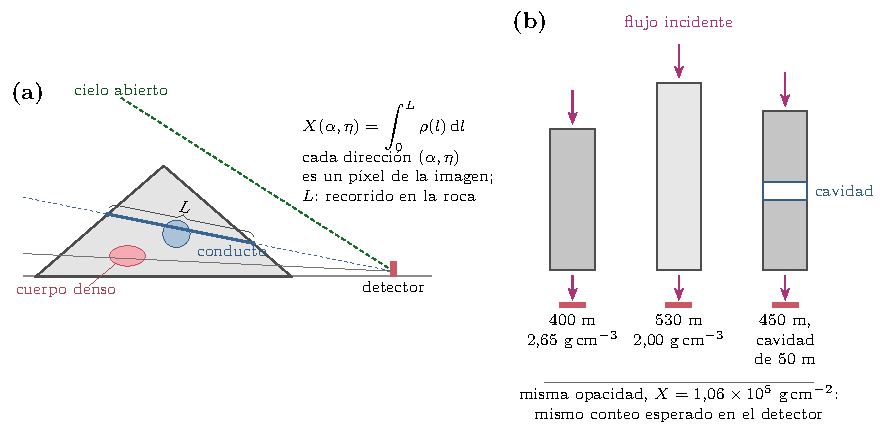
\includegraphics[width=\linewidth]{fig2-1_opacidad_proyeccion.pdf}
\caption[La imagen muográfica por transmisión como proyección]{La imagen muográfica por transmisión como proyección (esquema sin escala). (a)~Cada dirección $(\alpha,\eta)$ define un trayecto; el píxel correspondiente depende de la opacidad $X$ acumulada a lo largo del recorrido $L$ en la roca, incluidas las anomalías que encuentre, y la dirección de cielo abierto sirve de referencia para la transmisión. (b)~Ambigüedad entre espesor y densidad: 400~m de roca de 2,65~g\,cm$^{-3}$, 530~m de roca de 2,00~g\,cm$^{-3}$ y 450~m de roca de 2,65~g\,cm$^{-3}$ con una cavidad de 50~m tienen la misma opacidad, $1{,}06\times10^{5}$~g\,cm$^{-2}$, y producen el mismo conteo esperado. Fuente: elaboración de los autores.}
\label{fig:mt-proyeccion}
\end{figure}

De esa propiedad se siguen dos consecuencias. La primera es que el problema inverso no tiene solución única. Como muestra el panel~(b) de la \cref{fig:mt-proyeccion}, distribuciones de densidad diferentes producen la misma opacidad y, por tanto, el mismo conteo esperado: una roca delgada y densa equivale a una gruesa y liviana, y una cavidad puede compensarse con un trayecto más largo. Convertir una opacidad en densidad media exige conocer la longitud del recorrido, y recuperar la distribución tridimensional exige combinar varias vistas o información adicional \parencite{lechmann2021,tanaka2023muography}. La segunda consecuencia es que la interpretación se apoya en contrastes. Se compara el conteo de una región con el de otra región de referencia cuyo trayecto sea comparable, y una diferencia de conteo se atribuye a una diferencia de densidad solo si los trayectos comparados tienen longitudes semejantes; de lo contrario, una diferencia de longitud produce por sí sola una diferencia de opacidad.

Las \cref{eq:mt-tasa,eq:mt-transmision} muestran, además, que la relación entre conteos y opacidad no es lineal: depende del espectro del flujo, del ángulo cenital y de la pérdida de energía. Un contraste de conteos entre dos regiones es, por ello, una magnitud adimensional distinta de una diferencia de opacidad, que se expresa en g\,cm$^{-2}$. Pasar de uno a otra requiere un modelo de respuesta que relacione los conteos esperados con el flujo, la opacidad y la detección, o una calibración equivalente \parencite{lesparre2010}.

% =============================================================================
\section{Estadística de conteo y exposición}
\label{sec:mt-estadistica}

La llegada de muones a una celda angular es una sucesión de eventos independientes y raros, que se modela como un proceso de Poisson. Si la tasa $\lambda$ es constante, el número de muones $N(t)$ registrados durante una exposición $t$ sigue la distribución de la \cref{eq:mt-poisson-pmf}; su valor esperado y su varianza coinciden, como expresa la \cref{eq:mt-poisson-media}, y su ruido relativo es el de la \cref{eq:mt-poisson-relativo}:
\begin{subequations}\label{eq:mt-poisson}
\begin{align}
P\big(N(t)=n\big)&=\frac{(\lambda t)^{n}\,\mathrm e^{-\lambda t}}{n!},\qquad n=0,1,2,\ldots,\label{eq:mt-poisson-pmf}\\
\mathbb E[N(t)]&=\operatorname{Var}[N(t)]=\lambda t,\label{eq:mt-poisson-media}\\
\frac{\sqrt{\operatorname{Var}[N(t)]}}{\mathbb E[N(t)]}&=\frac{1}{\sqrt{\lambda t}}.\label{eq:mt-poisson-relativo}
\end{align}
\end{subequations}
En estas expresiones, $\lambda$ se expresa en s$^{-1}$ y $t$ en s, de modo que $\mu=\lambda t$, el número esperado de cuentas, es adimensional. La señal crece en proporción a la exposición y la desviación estándar solo con su raíz cuadrada. En consecuencia, el cociente entre la media y la desviación estándar de un conteo es $\sqrt{\mu}$ y el ruido relativo de la \cref{eq:mt-poisson-relativo} es $1/\sqrt{\mu}$, como muestra la \cref{fig:mt-ruido}. Un conteo con un valor esperado de cien cuentas fluctúa típicamente un 10\,\%, y uno de diez mil, un 1\,\%; reducir el ruido relativo a la mitad exige cuadruplicar la exposición. Este cociente estadístico de un conteo debe distinguirse de los indicadores espaciales que comparan la media de una región con la dispersión de sus píxeles, en los que la dispersión contiene también la estructura de la escena.

\begin{figure}[htbp]
\centering
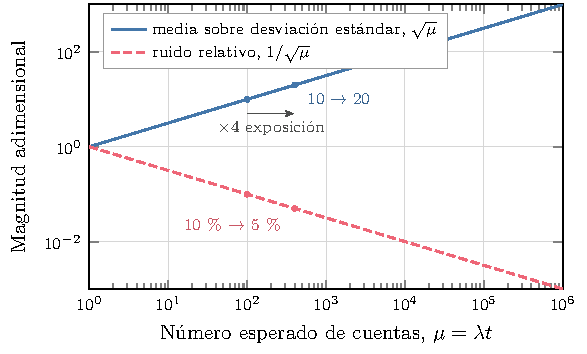
\includegraphics{fig2-2_ruido_conteo.pdf}
\caption[Media sobre desviación estándar y ruido relativo de un conteo de Poisson]{Cociente entre media y desviación estándar, $\sqrt{\mu}$, y ruido relativo, $1/\sqrt{\mu}$, de un conteo de Poisson en función de su valor esperado $\mu=\lambda t$, en escalas logarítmicas. Los puntos ilustran que cuadruplicar la exposición, de $\mu=100$ a $\mu=400$, duplica el cociente y reduce el ruido relativo del 10 al 5\,\%. Curvas analíticas, sin datos del proyecto. Fuente: elaboración de los autores.}
\label{fig:mt-ruido}
\end{figure}

De lo anterior se sigue una precisión sobre la expresión \emph{alta estadística}. Una imagen de alta estadística no es una imagen sin azar, sino una con muchos conteos por píxel y, por tanto, con ruido relativo pequeño pero no nulo. Cuando una imagen de larga exposición se usa como referencia para juzgar otra, la referencia conserva sus propias fluctuaciones estadísticas; por ello, coincidir con ella no equivale a recuperar una imagen libre de ruido.

El proceso de Poisson tiene una propiedad que permite estudiar exposiciones menores a partir de una sola medición o simulación. Si cada evento de un proceso de Poisson se conserva de manera independiente con probabilidad $f$, los eventos conservados forman de nuevo un proceso de Poisson, con la tasa multiplicada por $f$ \parencite{kingman1992}. En términos de conteos, la \cref{eq:mt-adelgazamiento} expresa este adelgazamiento binomial:
\begin{equation}\label{eq:mt-adelgazamiento}
N\sim\operatorname{Poisson}(\lambda t),\quad L\mid N\sim\operatorname{Binomial}(N,f)\;\Longrightarrow\;L\sim\operatorname{Poisson}(f\lambda t),
\end{equation}
donde $L$ es el conteo conservado y $f$, con $0<f\le1$, la fracción de conservación, ambos adimensionales. Como $f\lambda t$ es el valor esperado que correspondería a una exposición $ft$, el adelgazamiento produce, a partir de una imagen de exposición $t$, imágenes con la distribución marginal que tendrían mediciones de exposición $ft$, y la razón $1/f$ describe la reducción nominal de la exposición. La equivalencia vale para cada imagen por separado: las imágenes reducidas obtenidas de una misma imagen original comparten sus eventos y no son mediciones independientes entre sí ni de la original.

La estadística de conteo interviene también en el control de una proporción. Cuando de $N$ eventos se observa que $K$ cumplen una condición, la proporción estimada $K/N$ tiene una incertidumbre binomial, y el intervalo de Clopper y Pearson, construido a partir de los cuantiles de la distribución beta, garantiza una cobertura no menor que la nominal sin recurrir a aproximaciones normales \parencite{clopper1934}. Cuando se examinan simultáneamente muchas proporciones, la probabilidad de que alguno de los intervalos no contenga su valor verdadero crece con su número; la corrección de Bonferroni reparte el nivel de error entre las comparaciones para conservar una cobertura conjunta, a costa de intervalos más anchos \parencite{dunn1961}.

Por último, los conteos de una imagen muográfica abarcan varios órdenes de magnitud entre las direcciones de cielo abierto y las que atraviesan grandes espesores de roca. Una transformación logarítmica comprime ese intervalo dinámico, de modo que diferencias relativas iguales ocupen intervalos semejantes, y una transformación acotada permite representar los conteos en un intervalo finito adecuado para la salida de una red neuronal. Como toda transformación no lineal, cambia la escala de los errores: una discrepancia pequeña en el dominio transformado puede corresponder a una discrepancia grande en cuentas, en particular donde los conteos son altos, por lo que los errores deben examinarse en ambos dominios.

% =============================================================================
\section{Simulación Monte Carlo del transporte de muones}
\label{sec:mt-simulacion}

La muografía de campo no proporciona pares de imágenes de baja y alta estadística de un mismo objeto con estructura interna conocida: una medición real no tiene una versión equivalente sin ruido, y su estructura verdadera no se conoce. La simulación Monte Carlo resuelve esa carencia, porque produce imágenes de exposición controlada sobre escenarios cuya geometría y cuyos materiales se fijan de antemano. El método consiste en muestrear aleatoriamente las partículas primarias y los procesos físicos que cada una sufre a lo largo de su trayectoria, y en estimar las magnitudes de interés a partir de muchas historias independientes; la precisión de esas estimaciones está limitada por la estadística de conteo de la \cref{sec:mt-estadistica}.

Geant4 es un conjunto de herramientas de propósito general para simular el paso de partículas por la materia. Proporciona la descripción de la geometría y de los materiales, el seguimiento paso a paso de las partículas y el registro de las magnitudes de interés \parencite{agostinelli2003,allison2016}. Los procesos físicos se agrupan en listas de física, que combinan modelos electromagnéticos y hadrónicos validados para distintos intervalos de energía; la lista FTFP\_BERT, por ejemplo, emplea el modelo de cuerdas de Fritiof a energías altas y la cascada intranuclear de Bertini a energías bajas, junto con la física electromagnética estándar \parencite{allison2016}. Geant4 define además un corte de producción, expresado como una distancia, por debajo del cual no se generan partículas secundarias explícitas y su energía se deposita de forma continua. Ese corte controla el detalle de la simulación y no equivale a un umbral de energía para registrar las partículas que alcanzan una superficie de observación. Los materiales pueden tomarse de una base de datos de referencia, como el aire normalizado de Geant4, o definirse por su composición y densidad.

Las partículas primarias deben generarse según el flujo de la \cref{sec:mt-muones}. EcoMug es un generador de muones cósmicos que lo hace a partir de parametrizaciones del flujo medido y con distintas superficies de generación, lo que permite muestrear eficientemente momentos y direcciones \parencite{pagano2021}. Como la mayoría de los muones generados no atraviesa la roca o no llega a la región de observación, la eficiencia del muestreo condiciona el costo computacional de una campaña de simulación muográfica.

La simulación tiene, sin embargo, un límite epistemológico. Un modelo entrenado con datos simulados aprende la distribución de esos datos, y su desempeño sobre datos reales depende de la semejanza entre ambas distribuciones. En la muografía, la brecha entre simulación y realidad tiene varias fuentes: los detectores reales tienen eficiencia menor que la unidad, aceptancia y resolución angular finitas y un fondo de partículas que no son muones transmitidos, cuyo peso relativo crece donde la señal es menor \parencite{lesparre2010,lechmann2021}; los volcanes reales tienen topografía irregular y una estructura de densidades heterogénea, y las simulaciones simplificadas pueden omitir partículas secundarias o el detalle de la respuesta instrumental. El desempeño medido sobre escenarios simulados excluidos del entrenamiento describe, por tanto, la generalización dentro de la familia simulada y no garantiza por sí solo el comportamiento ante observaciones de campo.

% =============================================================================
\section{Aprendizaje profundo para la mejora de imágenes}
\label{sec:mt-aprendizaje}

Para una misma configuración de adquisición y un flujo estable, aumentar la exposición reduce el ruido relativo de conteo. La alternativa computacional consiste en estimar, a partir de la imagen ruidosa, la imagen que se habría obtenido con más exposición. En el aprendizaje supervisado, esa estimación se obtiene ajustando los parámetros $\theta$ de una función $G_\theta$ a un conjunto de pares formados por una entrada degradada $\boldsymbol u$ y su referencia $\boldsymbol y$, de modo que la salida $G_\theta(\boldsymbol u)$ se aproxime a $\boldsymbol y$ según una función de pérdida. Los parámetros se ajustan con variantes del descenso de gradiente estocástico sobre lotes de ejemplos; el método Adam adapta el paso de cada parámetro a partir de estimaciones de los momentos primero y segundo de su gradiente \parencite{kingma2015}.

Un modelo con muchos parámetros puede ajustarse a las particularidades de los datos de entrenamiento sin generalizar a casos nuevos. Por ello, el desempeño se juzga en un conjunto de validación no usado para ajustar los parámetros, que sirve para elegir el estado del modelo y detener el entrenamiento, y la estimación final se obtiene en un conjunto de prueba reservado. Esa separación solo es informativa si ningún dato del conjunto reservado influye en el entrenamiento: cuando las muestras están agrupadas, por ejemplo varias imágenes derivadas de un mismo escenario, repartir muestras de un mismo grupo entre entrenamiento y evaluación produce una fuga de información que sobrestima el desempeño, y la partición debe hacerse por grupos completos \parencite{kaufman2012}.

Las redes neuronales convolucionales son la arquitectura habitual para transformar imágenes. Cada capa aplica filtros aprendidos que recorren la imagen con pesos compartidos, seguidos de funciones de activación no lineales y, con frecuencia, de una normalización de las activaciones; la red detecta así un mismo patrón en cualquier posición. Al encadenar capas y reducir la resolución, cada salida depende de una región creciente de la entrada, llamada campo receptivo, y la red construye representaciones de escala cada vez mayor. La arquitectura U-Net organiza esas capas en un codificador, que reduce la resolución y captura el contexto, y un decodificador, que la recupera, unidos por conexiones de salto que transmiten directamente los detalles finos de cada escala \parencite{ronneberger2015}. Esa estructura resulta adecuada para transformar una imagen en otra del mismo tamaño.

La función de pérdida condiciona el tipo de estimación. Cuando varias referencias son compatibles con una misma entrada ruidosa, minimizar el error cuadrático conduce a su media condicional y minimizar el error absoluto, la pérdida $\mathcal L_1$, a su mediana. Ambas estimaciones promedian las estructuras posibles en lugar de elegir una de ellas y tienden, por ello, a producir imágenes suaves \parencite{isola2017}. Las redes generativas antagónicas se propusieron como una alternativa para aprender distribuciones de datos. En ellas, un generador $G_\theta$ produce muestras y un discriminador $D_\phi$ aprende a distinguirlas de los datos reales; ambos se entrenan como adversarios en el juego de la \cref{eq:mt-gan} \parencite{goodfellow2014}:
\begin{equation}\label{eq:mt-gan}
\min_{\theta}\max_{\phi}\;\mathbb E_{\boldsymbol y\sim p_{\mathrm{datos}}}\big[\log D_\phi(\boldsymbol y)\big]+\mathbb E_{\boldsymbol z\sim p_{\boldsymbol z}}\big[\log\big(1-D_\phi(G_\theta(\boldsymbol z))\big)\big],
\end{equation}
donde $p_{\mathrm{datos}}$ es la distribución de los datos reales, $\boldsymbol z$ una variable aleatoria con distribución $p_{\boldsymbol z}$ y $D_\phi(\cdot)\in(0,1)$ la probabilidad, estimada por el discriminador, de que su argumento provenga de los datos; todas las magnitudes son adimensionales. En la versión condicional, generador y discriminador reciben además una información de entrada, de modo que el generador aprende una distribución condicionada por ella \parencite{mirza2014}. Para la traducción entre imágenes, \textcite{isola2017} combinaron un generador U-Net condicionado por la imagen de entrada con un discriminador que recibe el par formado por la entrada y una imagen real o generada y juzga parches locales en lugar de la imagen completa, y añadieron un término $\mathcal L_1$ que mantiene la salida próxima a la referencia. El tamaño del parche juzgado corresponde al campo receptivo del discriminador y es una propiedad de la arquitectura, no una resolución física.

El entrenamiento antagónico es inestable cuando las distribuciones de los datos reales y generados apenas se solapan. \textcite{arjovsky2017} propusieron sustituir la divergencia implícita en la \cref{eq:mt-gan} por la distancia de Wasserstein, que sigue siendo informativa en ese caso y que, por la dualidad de Kantorovich y Rubinstein, se expresa como en la \cref{eq:mt-wasserstein}:
\begin{equation}\label{eq:mt-wasserstein}
W\big(P_{\boldsymbol y},P_{\widehat{\boldsymbol y}}\big)=\sup_{\|D\|_{L}\le1}\;\mathbb E_{\boldsymbol y\sim P_{\boldsymbol y}}\big[D(\boldsymbol y)\big]-\mathbb E_{\widehat{\boldsymbol y}\sim P_{\widehat{\boldsymbol y}}}\big[D(\widehat{\boldsymbol y})\big],
\end{equation}
donde $P_{\boldsymbol y}$ y $P_{\widehat{\boldsymbol y}}$ son las distribuciones de las referencias y de las salidas del generador, y el supremo se toma sobre las funciones $D$ con constante de Lipschitz $\|D\|_L$ no mayor que uno. El discriminador deja de estimar una probabilidad y se convierte en un crítico que asigna puntuaciones reales, cuya diferencia media aproxima la distancia. \textcite{gulrajani2017} impusieron la restricción de Lipschitz mediante una penalización que lleva hacia uno la norma del gradiente del crítico en puntos interpolados al azar entre referencias y salidas generadas, en lugar de recortar sus pesos; en la práctica, el crítico se actualiza varias veces por cada actualización del generador para que su estimación de la distancia sea informativa. La \cref{fig:mt-gan} reúne estos elementos en el caso condicional: el generador recibe la entrada, el crítico evalúa pares condicionados por ella mediante puntuaciones por parche y el generador se ajusta para reducir a la vez la discrepancia con la referencia y la separación que el crítico establece entre pares reales y generados.

\begin{figure}[htbp]
\centering
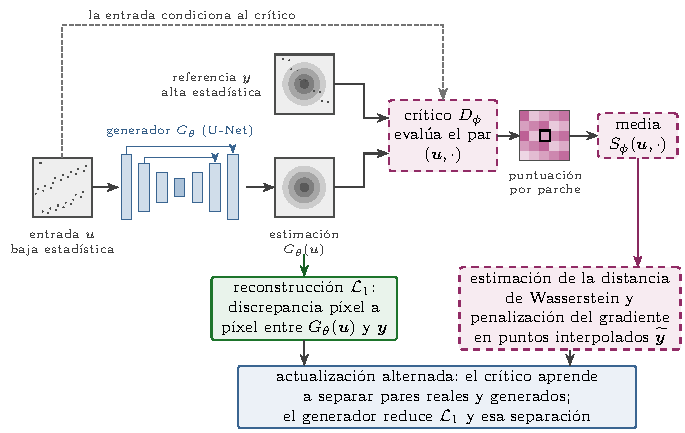
\includegraphics[width=\linewidth]{fig2-3_gan_condicional.pdf}
\caption[Esquema conceptual de una red generativa antagónica condicional de Wasserstein]{Esquema conceptual de una red generativa antagónica condicional de Wasserstein con crítico de parches. El generador $G_\theta$ transforma la entrada $\boldsymbol u$; el crítico $D_\phi$ puntúa por parches el par formado por la entrada y una imagen real o generada, y la media $S_\phi$ resume esas puntuaciones. El término $\mathcal L_1$ mide la discrepancia con la referencia $\boldsymbol y$ y la penalización del gradiente se evalúa en puntos interpolados $\widetilde{\boldsymbol y}$. Esquema sin dimensiones de capas. Fuente: elaboración de los autores a partir de \textcite{isola2017} y \textcite{gulrajani2017}.}
\label{fig:mt-gan}
\end{figure}

% =============================================================================
\section{Métricas de calidad y conservación}
\label{sec:mt-metricas}

Juzgar si una imagen estimada se aproxima a su referencia exige métricas de referencia completa, que comparan ambas imágenes píxel a píxel o en ventanas locales. El error cuadrático medio promedia las diferencias al cuadrado, y la relación señal-ruido de pico, PSNR, lo expresa en decibelios respecto del valor máximo de la representación; ambas miden la fidelidad punto a punto y son sensibles a cualquier diferencia de amplitud. El índice de similitud estructural, SSIM, compara en ventanas locales la luminancia, el contraste y la estructura de las dos imágenes, con la motivación de aproximarse a la percepción humana de la calidad \parencite{wang2004}. Ambas medidas responden de forma diferente a distintos tipos de degradación y conviene informarlas juntas \parencite{hore2010}. Las dos dependen, además, de la representación en que se calculan: evaluadas sobre conteos transformados, describen la similitud en esa escala y no la conservación de las cuentas.

La mejora de la similitud no basta para caracterizar una estimación. \textcite{blau2018} demostraron que la distorsión de una estimación, medida por su distancia a la referencia, y su calidad perceptual, medida por la proximidad de su distribución a la de las imágenes reales, no pueden optimizarse simultáneamente más allá de cierto límite. Una estimación de distorsión mínima tiende a ser suave, y una de apariencia realista tiende a alejarse más de la referencia; una red entrenada solo con error absoluto y una red antagónica ocupan, por ello, puntos distintos de ese compromiso, y ninguna métrica aislada basta para compararlas. Un suavizado, además, puede elevar la similitud global y reducir la dispersión de una región mientras atenúa una anomalía.

En la muografía, cada valor de píxel es un conteo con significado físico, ligado a la opacidad por la \cref{eq:mt-imagen}, y las métricas globales promedian sobre la imagen sin distinguir las regiones relevantes para la interpretación. La evaluación de una estimación muográfica requiere, por ello, medidas físicamente motivadas. El sesgo de las cuentas integradas en una región indica si la estimación conserva la información de transmisión; al permitir que excesos y déficits se compensen, se complementa con el error absoluto acumulado en la región, que distingue la conservación de la suma de la fidelidad espacial. La franja del contorno del edificio merece un tratamiento propio, porque allí los gradientes de conteo son mayores y la dispersión múltiple ya difumina la transición (\cref{sec:mt-muones}). El contraste de conteos de una anomalía respecto de regiones de control con trayectos comparables expresa la magnitud con la que se interpreta una imagen muográfica (\cref{sec:mt-imagen}), y su signo indica si la anomalía aparece como exceso o déficit de muones. Los indicadores que comparan la media de una región con la dispersión espacial de sus píxeles o de su fondo describen la intensidad y el contraste locales, pero no constituyen probabilidades de detección, porque esa dispersión contiene tanto fluctuaciones de conteo como estructura de la escena.

% =============================================================================
\section{Aprendizaje profundo en muografía}
\label{sec:mt-estado-arte}

El aprendizaje automático se ha incorporado a la muografía en varios puntos de la cadena de obtención de imágenes. La revisión de \textcite{luo2025} organiza las técnicas de reconstrucción en imagen por dispersión, por transmisión y con partículas secundarias, y examina para la transmisión las limitaciones del método basado en la razón de flujos frente a algoritmos de inversión de densidad. En la etapa del detector, \textcite{galgoczi2024} entrenaron una red neuronal profunda con muestras simuladas para suprimir el fondo de baja energía en un sistema orientado a la muografía de volcanes, un problema que el telescopio colombiano MuTe aborda con instrumentación híbrida \parencite{penarodriguez2020}. En la tomografía por dispersión, que reconstruye volúmenes pequeños a partir de la desviación de cada muon, se han desarrollado marcos de reconstrucción diferenciables \parencite{sattler2025} y redes convolucionales que reducen el ruido de las reconstrucciones \parencite{vinodkumar2025}, y \textcite{wang2026} aplicaron una U-Net entrenada con simulaciones a datos experimentales de exposición corta.

En la mejora de imágenes de baja estadística, los antecedentes son más escasos. \textcite{lefevre2024} entrenaron con muografías simuladas una red para reducir el ruido estadístico de imágenes obtenidas con detectores Micromegas, y \textcite{odonnell2025particles} aplicaron una red generativa antagónica condicional de Wasserstein con penalización de gradiente a la mejora de imágenes muográficas de estructuras de concreto, con imágenes de un día de exposición que alcanzaron, según el SSIM, la calidad de imágenes de 21 días. En un problema estadísticamente análogo, la tomografía computarizada de baja dosis, cuyo ruido cuántico también es de Poisson, \textcite{yang2018} mostraron que una red antagónica con distancia de Wasserstein preserva texturas que una pérdida de error cuadrático tiende a suavizar. Las aplicaciones volcánicas de la muografía, por su parte, se han apoyado en mapas bidimensionales de opacidad y en sus contrastes \parencite{tanaka2007asama,olah2018sakurajima,tanaka2023muography}. En la literatura revisada no se identificó la aplicación de redes generativas condicionales a la mejora de imágenes de baja estadística de edificios volcánicos, un escenario cuyas distancias, espesores y contrastes difieren de los de las estructuras civiles y de los volúmenes de la tomografía por dispersión, y cuyo entrenamiento exige, como en los trabajos citados, datos simulados.

Con estos elementos quedan establecidos los fundamentos que la metodología requiere: la física que liga los conteos con la opacidad, la estadística que limita su calidad y permite reducir la exposición de forma controlada, la simulación que produce escenarios de estructura conocida, los modelos capaces de estimar imágenes de mayor estadística y los criterios con los que debe juzgarse el resultado. El \cref{chap:metodologia} describe cómo se aplicaron.
